\documentclass{beamer}

\usepackage{amsmath}
\usepackage{amsfonts}
\usepackage{amssymb}
\usepackage{listings}
\usepackage{graphicx}
\usepackage{tikz}

\graphicspath{{../}}

% KCPC theme
\usetheme{default}
\useinnertheme{rectangles}
\useoutertheme{default}

\beamerdefaultoverlayspecification{<+->}

\setbeamertemplate{navigation symbols}{}

% Colours
\definecolor{kcpc-bg}{RGB}{250,250,250}
\definecolor{kcpc-text}{RGB}{20,20,20}
\definecolor{kcpc-muted}{RGB}{90,90,90}
\definecolor{kcpc-red}{RGB}{176,0,0}

\setbeamercolor{background canvas}{bg=kcpc-bg}
\setbeamercolor{normal text}{fg=kcpc-text}
\setbeamercolor{frametitle}{fg=kcpc-text,bg=kcpc-bg}
\setbeamercolor{title}{fg=kcpc-text}
\setbeamercolor{subtitle}{fg=kcpc-muted}
\setbeamercolor{structure}{fg=kcpc-red}

\setbeamerfont{title}{series=\bfseries,size=\Large}
\setbeamerfont{frametitle}{series=\bfseries,size=\large}

\setlength{\parskip}{0.4em}

\setbeamertemplate{itemize item}{$\rightarrow$}
\setbeamertemplate{itemize subitem}{$\rightarrow$}

\setbeamertemplate{headline}{
    \vspace{0.2cm}
    \hspace{0.2cm}
    \textcolor{kcpc-muted}{\small\insertsection}
    \hfill
}

\setbeamertemplate{footline}{
    \hspace{0.2cm}
    \textcolor{kcpc-muted}{\small KCPC}
    \hfill
    \vspace{0.3cm}
}

\setbeamertemplate{background}{
    \begin{tikzpicture}[remember picture,overlay]
        \node[
            opacity=0.035,
            at=(current page.center)
        ] {
            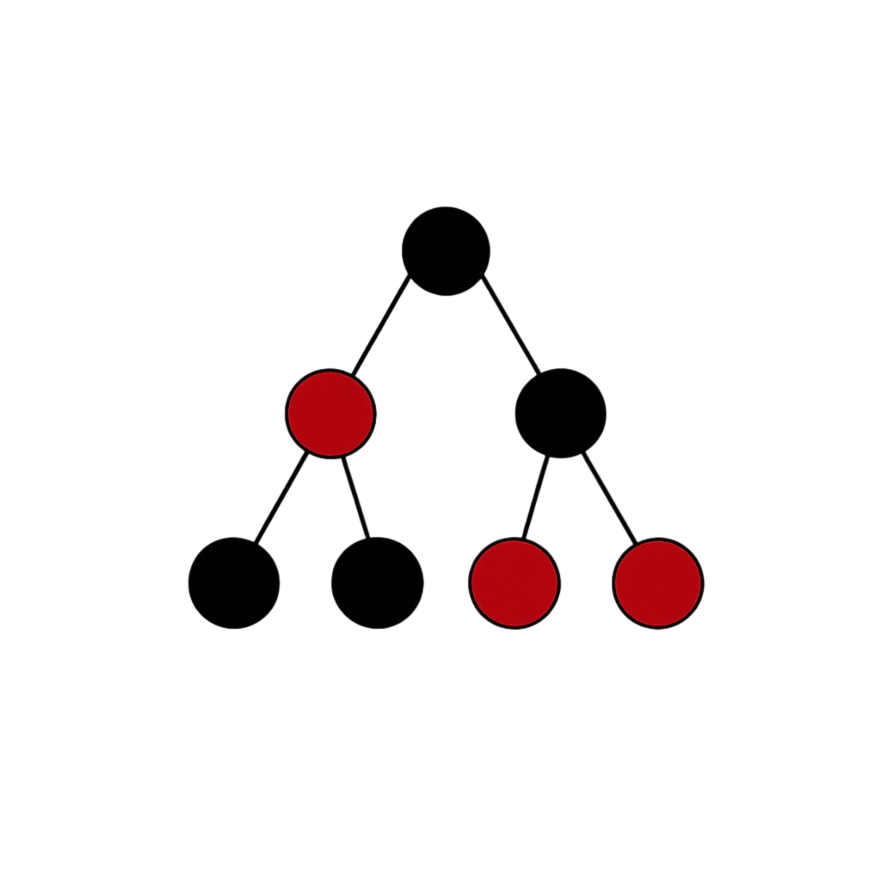
\includegraphics[width=0.55\paperwidth]{kcpc-logo.png}
        };
    \end{tikzpicture}
}

\AtBeginSection[]{
    \begin{frame}[plain]
        \vfill
        \centering
        {\Large\bfseries \insertsection}
        \vfill
    \end{frame}
}

\title{Mathematical Problem Solving II}
\subtitle{Advanced Invariants, Heuristics, and Algorithmic Thinking}
\author{KCPC}
\date{Week 2}

\newcommand{\concept}[1]{\textbf{Concept:} #1}
\newcommand{\apply}[1]{\textbf{How it applies:} #1}
\newcommand{\heuristic}[1]{\textbf{Heuristic:} #1}

\begin{document}

\begin{frame}
    \titlepage
\end{frame}

\begin{frame}{Overview}
    \tableofcontents
\end{frame}

\section{Week 1 Recap and What Comes Next}

\begin{frame}{Week 1 Recap}
    Last week we built a toolkit for reasoning about puzzles:
    \pause
    \begin{itemize}
        \item Logic: track knowledge, what is true, what is inferred.
        \item Invariants: find what cannot change; prove impossibility.
        \item Colouring: turn geometry into counting.
        \item Induction: reduce the problem size step by step.
        \item Monovariants: track progress towards a goal.
    \end{itemize}
\end{frame}

\begin{frame}{Heuristics}
    \pause
    \begin{itemize}
        \item Wishful thinking: simplify the problem; assume a nice form.
        \item Symmetry: pair objects; look for transformations that leave
            the problem unchanged.
        \item Extreme principle: focus on the most extreme object.
        \item Reduction: change representation to expose structure.
    \end{itemize}
\end{frame}

\begin{frame}{This Week: Deeper Tools And Algorithmic Bridges}
    \begin{itemize}
        \item Strengthen each Week 1 tool with harder problems and
            generalisations.
        \item See how mathematical insight becomes an algorithmic idea.
        \item Practise the full cycle: model, reason, implement, verify.
        \item Connect to standard CP platforms: CSES, Codeforces, AtCoder.
    \end{itemize}
\end{frame}

\section{Advanced Logic And Common Knowledge}

\begin{frame}{Logic Beyond Two Doors}
    \concept{Common knowledge is what everyone knows, everyone knows
    everyone knows, etc.}

    \begin{itemize}
        \item Public announcements change the state of knowledge.
        \item Reasoning depth: ``I know that you know that I know...''
        \item Often reduces to a fixed-point: when no new deductions
            are possible.
    \end{itemize}
\end{frame}

\begin{frame}{Worked Example: Muddy Children (Public Announcement)}
    $n$ children play outside. $k$ of them have mud on their foreheads.
    Each sees the others but not themselves.

    Father announces: ``At least one of you has mud.'' Then he
    repeatedly asks: ``Does anyone know their own state?''

    \vspace{0.5em}
    What happens?
\end{frame}

\begin{frame}{Muddy Children: Applying The Concept}
    \apply{Induction on the number of muddy children $k$.}

    \begin{itemize}
        \item If $k=1$: that child sees no mud, knows they must be the
            one. Answers yes on round 1.
        \item If $k=2$: each sees one muddy child. If I were clean, the
            other would see 0 and answer on round 1. They don't. So I must
            be muddy. Both answer on round 2.
        \item Induction: if $k$, all $k$ answer on round $k$.
    \end{itemize}
\end{frame}

\begin{frame}{Student Exercises: Advanced Logic}
    \begin{itemize}
        \item Basic: Blue-Eyed Islanders (public announcement, $k=2$).
        \item Easy: Cheating Husbands (induction on public knowledge).
        \item Medium: Sum and Product Puzzle (Freudenthal's problem).
        \item Hard: Cheryl's Birthday (iterated elimination).
        \item Very Hard: 100 Prisoners and a Light Bulb (protocol design).
    \end{itemize}
\end{frame}

\section{Advanced Invariants And Monovariants}

\begin{frame}{Generalising Invariants}
    \concept{An invariant can be a number, a parity, a polynomial, a
    vector modulo $m$, or a potential function.}

    \begin{itemize}
        \item Modulo invariants: track values mod $2, 3, 4, \ldots$
        \item Polynomial invariants: e.g., $x^2+y^2$ for rotation.
        \item Potential functions: sum of weights that never increases.
        \item Multiple invariants together can prove stronger results.
    \end{itemize}
\end{frame}

\begin{frame}{Worked Example: Peg Solitaire}
    On a cross-shaped board, a peg jumps over an adjacent peg into an
    empty hole, removing the jumped peg.

    Can a single peg be moved to the centre from the standard starting position?
\end{frame}

\begin{frame}{Peg Solitaire: Applying The Concept}
    \apply{Assign weights to holes; total weight never increases.}

    \begin{itemize}
        \item Label each hole with a value from $\{1, x, x^2\}$ where $x$
            satisfies $x^2+x+1=0$.
        \item Any legal jump preserves the sum of values of occupied holes.
        \item Compute the initial sum and the target sum.
        \item They differ, so the target is unreachable.
    \end{itemize}
\end{frame}

\begin{frame}{Student Exercises: Advanced Invariants}
    \begin{itemize}
        \item Basic: Peg solitaire on a smaller board.
        \item Easy: Token game with modular invariant.
        \item Medium: Conway's Soldiers (checker jumping).
        \item Hard: Polynomial invariant for grid walks.
        \item Very Hard: Invariant for the IMO 1986 Problem 3
            (integer sequence).
    \end{itemize}
\end{frame}

\section{Colouring And Tiling: Generalisations}

\begin{frame}{Beyond Two Colours}
    \concept{Colouring with 3, 4, or more colours captures more structure.}

    \begin{itemize}
        \item Triominoes and 3-colourings.
        \item Tetrominoes and 4-colourings.
        \item Modular colourings: colour $(i,j)$ by $(i+j)\bmod m$ or
            $(i+2j)\bmod m$.
        \item Each tile shape interacts with colours in a predictable way.
    \end{itemize}
\end{frame}

\begin{frame}{Worked Example: Tiling With Trominoes}
    Can a $5\times8$ board be tiled by $2\times2$ squares and
    L-shaped trominoes?
\end{frame}

\begin{frame}{Tromino Tiling: Applying The Concept}
    \apply{Use a 4-colouring based on coordinates mod 2.}

    \begin{itemize}
        \item Colour each cell $(i,j)$ by $(i\bmod 2, j\bmod 2)$: four
            colour classes.
        \item A $2\times2$ square covers one of each colour.
        \item A tromino covers three different colours, missing one.
        \item Count how many cells of each colour the board has.
        \item The counts show tiling is impossible.
    \end{itemize}
\end{frame}

\begin{frame}{Student Exercises: Advanced Colouring}
    \begin{itemize}
        \item Basic: Tiling a deficient board with trominoes.
        \item Easy: 3-colouring for dominoes on a torus.
        \item Medium: Tiling with T-tetrominoes.
        \item Hard: Fault-free tilings.
        \item Very Hard: Generalised mutilated chessboard.
    \end{itemize}
\end{frame}

\section{Induction And Recursion: From Proof To Algorithm}

\begin{frame}{Induction As A Design Principle}
    \concept{If I can solve size $n$ using a solution for size $n-1$, I
    have a recursive algorithm.}

    \begin{itemize}
        \item Proof by induction $\leftrightarrow$ recursive function.
        \item Base case $\leftrightarrow$ terminating condition.
        \item Inductive step $\leftrightarrow$ recursive call and combination.
        \item Strong induction $\leftrightarrow$ divide-and-conquer or DP.
    \end{itemize}
\end{frame}

\begin{frame}{Worked Example: Tower Of Hanoi}
    Three pegs, $n$ disks of decreasing size. Move stack from peg A to peg C.
\end{frame}

\begin{frame}{Tower Of Hanoi: Applying The Concept}
    \apply{Recursive solution from induction on $n$.}

    \begin{itemize}
        \item Move top $n-1$ disks from A to B.
        \item Move largest disk from A to C.
        \item Move $n-1$ disks from B to C.
        \item Minimum moves: $2^n-1$ (prove by induction).
    \end{itemize}

    The recursive structure \emph{is} the algorithm.
\end{frame}

\begin{frame}{Student Exercises: Induction To Algorithm}
    \begin{itemize}
        \item Basic: Josephus problem (eliminate every second person).
        \item Easy: Gray codes (recursive construction).
        \item Medium: Recursive algorithm for the 15-puzzle parity.
        \item Hard: Optimal strategy for the counterfeit coin with
            $n$ weighings.
        \item Very Hard: Recursive construction of Hadamard matrices.
    \end{itemize}
\end{frame}

\section{Heuristics In Depth}

\begin{frame}{Wishful Thinking: Simplify Until Solvable}
    \heuristic{Assume the answer has a nice form. What would make this easy?}

    \begin{itemize}
        \item ``If only the numbers were smaller...''
        \item ``If only the constraints were simpler...''
        \item ``What would the solution look like if I already knew it?''
        \item Then find the reduction from the real problem to the
            simplified one.
    \end{itemize}
\end{frame}

\begin{frame}{Worked Example: Wishful Thinking -- Sum of Squares}
    Find all integer solutions to $x^2 + y^2 = 2z^2$ with $x,y,z > 0$.

    \vspace{0.5em}
    Wishful thinking: what if $x+y$ and $x-y$ had a nice structure?
\end{frame}

\begin{frame}{Wishful Thinking: Applying The Concept}
    \apply{Set $x = u+v$, $y = u-v$.}

    \begin{itemize}
        \item $x^2 + y^2 = (u+v)^2 + (u-v)^2 = 2u^2 + 2v^2 = 2z^2$.
        \item So $u^2 + v^2 = z^2$ -- a Pythagorean triple!
        \item All solutions: $u = m^2-n^2$, $v = 2mn$, $z = m^2+n^2$
            (or swapped).
        \item Then $x = (m^2-n^2) + 2mn$, $y = (m^2-n^2) - 2mn$.
    \end{itemize}
\end{frame}

\begin{frame}{Student Exercises: Wishful Thinking}
    \begin{itemize}
        \item<1-> Basic: Solve $x^2 + y^2 = z^2$ in positive integers.
        \item<1-> Easy: Find all $n$ such that $n^2 + (n+1)^2$ is a
            perfect square.
        \item<1-> Medium: $x^2 + y^2 + z^2 = 2xyz$ (use wishful
            thinking to reduce).
        \item<1-> Hard: Integer solutions to $a^2 + b^2 = 3c^2$.
        \item<1-> Very Hard: Parametrise rational points on $x^3 + y^3 = 9$.
    \end{itemize}
\end{frame}

\begin{frame}{Symmetry: Exploit Invariance Under Transformations}
    \heuristic{Look for operations that leave the problem unchanged.}

    \begin{itemize}
        \item Pairing strategy: if the opponent moves, reply symmetrically.
        \item Canonical form: transform to a standard representative.
        \item Symmetric positions often have symmetric optimal moves.
    \end{itemize}
\end{frame}

\begin{frame}{Worked Example: Symmetry -- Pairing Game}
    Two players alternately place a domino on a $4\times4$ board.
    Dominoes cannot overlap. The player who cannot move loses.
    Show the second player has a winning strategy.
\end{frame}

\begin{frame}{Symmetry: Applying The Concept}
    \apply{Mirror every move across the centre.}

    \begin{itemize}
        \item The $4\times4$ board is centrally symmetric.
        \item If the first player places a domino covering $(x,y)$
            and $(x',y')$,
            the second player places one covering the centrally
            symmetric squares.
        \item This move is always legal because the board was symmetric and the
            first player's move was legal.
        \item The second player never runs out of moves first, so wins.
    \end{itemize}
\end{frame}

\begin{frame}{Student Exercises: Symmetry}
    \begin{itemize}
        \item<1-> Basic: Pairing game on a $2\times n$ board.
        \item<1-> Easy: Symmetry strategy in Chomp (poisoned chocolate).
        \item<1-> Medium: Second player wins on even$\times$even board with
            centrally symmetric tiles.
        \item<1-> Hard: Symmetry in the game of Nim with paired heaps.
        \item<1-> Very Hard: Strategy stealing argument for Hex.
    \end{itemize}
\end{frame}

\begin{frame}{Extreme Principle: The Boundary Holds The Answer}
    \heuristic{Consider the largest, smallest, leftmost, rightmost, or
    most extreme object.}

    \begin{itemize}
        \item The extremal object has restricted neighbours.
        \item Often leads to contradiction or constructive greedy choice.
        \item Works in geometry, combinatorics, number theory, and algorithms.
    \end{itemize}
\end{frame}

\begin{frame}{Worked Example: Extreme Principle -- Points in a Circle}
    Given 5 points in a unit circle, prove that some pair is at distance
    $\le 1$.

    \vspace{0.5em}
    Consider the point farthest from the centre...
\end{frame}

\begin{frame}{Extreme Principle: Applying The Concept}
    \apply{Let $P$ be the point with maximum distance from the centre $O$.}

    \begin{itemize}
        \item Let $OP = r \le 1$. All points lie in the unit circle
            centred at $O$.
        \item The other 4 points lie in the intersection of the unit circle
            and the circle of radius $r$ centred at $P$.
        \item This intersection is contained in a circle of radius $r/2$...
        \item (Standard proof: divide into 5 sectors of $72^\circ$, or use
                the fact that the maximum minimum distance for 5 points in a
                unit circle is $2\sin(36^\circ) > 1$; the claim as stated needs
                unit circle of diameter 1. Adjusting: for 5 points in a circle
            of diameter 1, some pair is at distance $\le 1/2$.)
    \end{itemize}
\end{frame}

\begin{frame}{Student Exercises: Extreme Principle}
    \begin{itemize}
        \item<1-> Basic: 5 points in a unit square; some pair at distance
            $\le \sqrt{2}/2$.
        \item<1-> Easy: In any set of 10 integers, some subset sums to a
            multiple of 10 (consider extreme partial sums).
        \item<1-> Medium: Maximum area triangle inscribed in a circle is
            equilateral (extreme principle on area).
        \item<1-> Hard: In a tournament, there is a ``king'' (vertex
            distance $\le 2$ to all others).
        \item<1-> Very Hard: Sylvester-Gallai theorem (extreme point gives
            contradiction).
    \end{itemize}
\end{frame}

\begin{frame}{Reduction: Change The Representation}
    \heuristic{Replace the problem with an equivalent one that is
    easier to see.}

    \begin{itemize}
        \item Graph modelling: vertices and edges instead of story.
        \item Algebraic encoding: variables and equations instead of logic.
        \item Modulo arithmetic: finite states instead of infinite.
        \item This is the bridge to competitive programming.
    \end{itemize}
\end{frame}

\begin{frame}{Worked Example: Reduction -- Lamps in a Circle}
    $n$ lamps in a circle, each on or off. A move toggles lamp $i$ and
    its two neighbours. From a given configuration, can you reach all off?
\end{frame}

\begin{frame}{Reduction: Applying The Concept}
    \apply{Model as linear algebra over $\mathbb{F}_2$.}

    \begin{itemize}
        \item State vector $v \in \mathbb{F}_2^n$. Move $i$ adds vector
            $m_i$ with 1s at positions $i-1, i, i+1$ (mod $n$).
        \item Reachable configurations from $v_0$ are $v_0 +
            \text{span}\{m_1,\ldots,m_n\}$.
        \item This is a linear subspace. All-off reachable iff $v_0$
            is in the span.
        \item For $n$ not divisible by 3, the moves are independent and span
            the whole space -- always solvable.
        \item For $n$ divisible by 3, the sum of all move vectors is 0, and
            the invariant is the sum of bits at positions
            $0,3,6,\ldots$ modulo 2.
    \end{itemize}
\end{frame}

\begin{frame}{Student Exercises: Reduction}
    \begin{itemize}
        \item<1-> Basic: Water jugs as graph reachability.
        \item<1-> Easy: Lights Out puzzle on a $3\times3$ grid.
        \item<1-> Medium: Reduce 15-puzzle parity to permutation sign.
        \item<1-> Hard: Reduction from subset sum to knapsack.
        \item<1-> Very Hard: Prove equivalence of two formulations of
            the same contest problem (reduction to known NP-complete problem).
    \end{itemize}
\end{frame}

\section{From Mathematical Insight To Algorithmic Thinking}

\begin{frame}{The Bridge To Competitive Programming}
    \begin{itemize}
        \item Mathematical proof $\to$ algorithm is often mechanical.
        \item The invariant \emph{is} the loop invariant.
        \item The induction \emph{is} the recursion or DP recurrence.
        \item The reduction \emph{is} the modelling step.
    \end{itemize}
\end{frame}

\begin{frame}{Modelling A Puzzle As A Graph (Algorithmic Bridge)}
    \concept{Many puzzles become graph reachability or shortest path.}

    \begin{itemize}
        \item State = complete description of the current situation.
        \item Edge = one legal move.
        \item Solution = path from start state to goal state.
        \item BFS finds the shortest solution.
        \item An invariant proves two states are in different components.
    \end{itemize}
\end{frame}

\begin{frame}{Worked Example: Water Jugs As A Graph}
    Two jugs of capacities 3 and 5. Target: measure exactly 4 units.
    Allowed: fill, empty, pour.

    \vspace{0.5em}
    States: $(a,b)$ where $0\le a\le3$, $0\le b\le5$.
    Edges: the six legal operations.
    BFS from $(0,0)$ to any state with $a=4$ or $b=4$.
\end{frame}

\begin{frame}{Greedy Choices From The Extreme Principle (Algorithmic Bridge)}
    \concept{The extreme principle often justifies a greedy choice.}

    \begin{itemize}
        \item Activity selection: earliest finish time is the extreme interval.
        \item Coin change (canonical systems): largest coin is the
            extreme choice.
        \item Fractional knapsack: highest value/weight ratio is the
            extreme item.
        \item Proof: exchange argument shows the extreme choice is safe.
    \end{itemize}
\end{frame}

\begin{frame}{Recurrence From Induction (Algorithmic Bridge)}
    \concept{Inductive proofs directly give recurrences.}

    \begin{itemize}
        \item Define $f(n)$ = answer for size $n$.
        \item Inductive step: $f(n) = \text{combination of } f(\text{smaller})$.
        \item Memoise or tabulate to avoid recomputation.
        \item This is dynamic programming.
    \end{itemize}
\end{frame}

\begin{frame}{Student Exercises: Algorithmic Bridges}
    \begin{itemize}
        \item Basic: BFS on water jug states (implement conceptually).
        \item Easy: Greedy activity selection from extreme principle.
        \item Medium: DP from induction: coin change / ways to make sum.
        \item Hard: State-space search for a sliding puzzle.
        \item Very Hard: Design and analyse a greedy algorithm for a
            scheduling problem.
    \end{itemize}
\end{frame}

\begin{frame}{Wrap-Up}
    Pair 1 complete: Logic, Invariants, Heuristics.
    \begin{itemize}
        \item Logic tracks knowledge; common knowledge enables coordination.
        \item Invariants prove impossibility; monovariants prove progress.
        \item Colouring turns geometry into arithmetic.
        \item Induction reduces problems; recursion builds algorithms.
        \item Heuristics: wishful thinking, symmetry, extreme, reduction.
    \end{itemize}

    Algorithmic bridges:
    \begin{itemize}
        \item State-space modelling $\to$ graph algorithms (Pair 3).
        \item Greedy from extreme principle $\to$ greedy algorithms (Pair 2/7).
        \item Induction to recurrence $\to$ dynamic programming (Pair 4/8).
    \end{itemize}

    Next: Pair 2 -- Core CP Fundamentals: Prefix Sums, Two Pointers,
    Binary Search.
\end{frame}

\end{document}
